\chapter{The effect of viscosity on the Kelvin-Helmholtz instability in the fan plane of a null point}

\graphicspath{{images/null_point_khi/}}

\section{Introduction}

\subsection{Why are nulls important?}

Flares, reconnection, etc

Note - these null point sims allow switching model to fulfil its destiny.

\section{Methods}

\subsection{Numerical setup}

\subsection{Tools of analysis}

There are three quantities useful in understanding the stability of the current-vortex sheet. Associated with the shear in velocity and magnetic field are two Mach numbers: the fast mode Mach number, related to the velocity shear, and the projected Alfv\'en Mach number, related to the magnetic shear,
\begin{equation}
  \label{eq:mach_numbers}
  M_f = \frac{\Delta v}{\sqrt{c_s^2 + c_A^2}} \text{and} \quad M_A = \frac{\Delta v \sqrt{rho}}{\Delta B},
\end{equation}
where $\Delta v$ and $\Delta B$ are the respective differences in the velocity and magnetic field over the shear layer, and $c_s$ and $v_A$ are the local sound and Alfv\'en speeds, respectively. Since the shear layer occurs in the presence of a guide field (that of the initial magnetic null point) which does not affect the linear stability of the KHI, we consider the Alfv\'en Mach number projected on to the layer. The parameter describing the balance of stability between the tearing mode and the KHI in a current-vortex sheet is
\begin{equation}
  \label{eq:khi_stability_param}
  \Gamma = \frac{L_b}{L_v} M_A^{2/3}
\end{equation}
where $L_b$ and $L_v$ are the respective widths of the magnetic and velocity shear layers~\cite{einaudiResistiveInstabilitiesFlowing1986}. Again, due to the presence of the guide field, we consider $\Gamma$ projected on to the shear layer. Plotting the radial dependence of these quantities over the shear layers gives an idea of the probable stability. It should be noted that the true stability of the current-vortex sheet studied here also depends on other factors not taken into account by the stability analysis performed by~\cite{einaudiResistiveInstabilitiesFlowing1986} (factors such as viscosity and the presence of a guide field). Hence, these quantities are only an indicator of the stability, not a guarantee.

\section{Results}

\subsection{Evolution of a typical KHI case}

We discuss initially the evolution of the simulations using a resistivity of $\eta = 10^{-4}$ and viscosity $\nu = 10^{-4}$, comparing the two viscosity models. This pair of simulations captures the main features of the null's response to the driver: the formation of a current-vortex sheet in the fan plane, the appearance of counterflows, the growth of a Kelvin-Helmholtz instability, and an eventual null collapse triggered by a fluting instability. This specific choice of parameters also highlights the differences between the isotropic and the switching viscosity models, mainly the suppression of the KHI in the isotropic case.

The total kinetic energy reveals the main developments in the simulations (Figure~\ref{fig:v-4r-4_kinetic_energy}). The initial acceleration of the drivers and injection of torsional Alfv\'en waves occurs between $t=0$ and $2$. After this time the effect of the viscosity models becomes apparent; the KHI grows only in the switching case, peaking between $t=9$ and $10$. Looking at only the switching case, the instability generates vortices in the fan plane, encouraging currents and enhanced Ohmic heating, converting some of the available kinetic energy to heat, which in turn results in a drop of kinetic energy between $t=10$ and $12$. The current sheets created during the instability also permit small reconnection events, indicated by small peaks in the kinetic energy between $t=10$ and $12$. After $t=12$, TODO. In contrast, without the triggering influence of the KHI the isotropic case becomes unstable to the fluting instability at a later time, resulting in a spike in kinetic energy associated with the collapse of the null point.

\begin{figure}[t]
  \centering
  \includegraphics[width=0.95\linewidth]{v-4r-4_kinetic_energy}
  \caption{}%
  \label{fig:v-4r-4_kinetic_energy}
\end{figure}

Initially, at $t=1$ the torsional Alfv\'en waves injected by the driver trace the field surrounding the null, moving towards the fan plane and out from the spine. The waves eventually meet and create an shear layer in the velocity and magnetic field in the form of a ring of vorticity and current density. Without any diffusion in the system the main wavefronts would travel far along the field before meeting. The presence of both viscosity and resistivity encourages the waves to diffuse as they travel along the field, allowing the upper and lower waves to meet relatively close to the spine, creating rings of shear which are both thicker and smaller in radius. In the switching case, due to the switching model diffusing the field less effectively than the isotropic model, the rings are typically larger in radius, stronger in magnitude, and thinner (Figure~\ref{fig:v-4r-4_vorticity_current_ring_t_3}). Since the viscosity diffuses velocity directly, and affects the magnetic field field through that, the vorticity is affected more than the current density.

\begin{figure}[t]
  \centering
  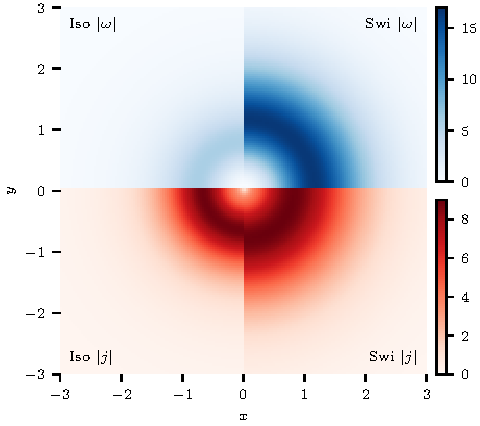
\includegraphics[width=0.48\linewidth]{v-4r-4_vorticity_current_ring_t_3}
  \caption{}%
  \label{fig:v-4r-4_vorticity_current_ring_t_3}
\end{figure}

In the switching case, the velocity shear layer becomes unstable to the KHI, initially presenting as a small, ring-like perturbation overlaying the velocity structure produced by boundary effects (Figure~\ref{fig:v-4r-4_vz_z_0_t_2}). The shear layers created in the isotropic case are do not have the required stability criteria[TODO expand on this or link back] (Figure~\ref{fig:v-4r-4_mach_t_2}). Between times $t=2$ and $6$ counterflows appear (Figure~\ref{fig:v-4r-4_counterflows_t_6}), opposite to the direction of the driver, and the current-vortex sheet grows in both size and magnitude, more in the switching case than the isotropic. The KHI also grows, still only in the switching case. At $t=6$, the reconnection rate is notably higher in the switching case, an indicator of more efficient slippage reconnection near the null TODO FIG line plot of reconnection rate over time.

\begin{figure}[t]
  \centering
  \includegraphics[width=0.8\linewidth]{v-4r-4_vz_z_0_t_2.pdf}
  \caption{}%
  \label{fig:v-4r-4_vz_z_0_t_2}
\end{figure}

\begin{figure}[t]
  \centering
  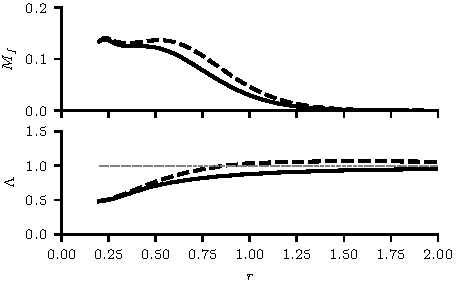
\includegraphics[width=0.9\linewidth]{v-4r-4_mach_t_2.pdf}
  \caption{}%
  \label{fig:v-4r-4_mach_t_2}
\end{figure}

\begin{figure}[t]
  \centering
  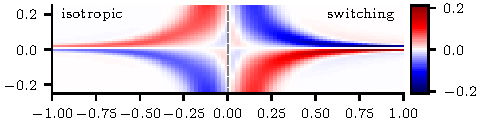
\includegraphics[width=0.9\linewidth]{v-4r-4_counterflows_t_6.pdf}
  \caption{}%
  \label{fig:v-4r-4_counterflows_t_6}
\end{figure}

At $t=7$ the KHI has visibly spread along the fan plane (Figure~\ref{fig:v-4r-4_vz_z_0_t_7}) and by $t=9$ it's clearly visible in the vorticity and current density (Figure~\ref{fig:v-4r-4_vorticity_current_ring_t_9}), although the diagonals are more pronounced, being strongly affected by the boundaries. Due to the shearing action of the counterflows, a secondary ring of strong current density has formed closer to the spine. The strength of the current density suggests reconnection may be being enhanced in the fan plane by the instability. Indeed, at $t=10$ a branching pattern in the field-integrated parallel electric field provides further evidence for reconnection occurring locally in the rolls of the KHI (Figure~\ref{fig:v-4r-4_reconn_rate_swi_t_10}).

\begin{figure}[t]
  \centering
  \includegraphics[width=0.8\linewidth]{v-4r-4_vz_z_0_t_7.pdf}
  \caption{}%
  \label{fig:v-4r-4_vz_z_0_t_7}
\end{figure}

\begin{figure}[t]
  \centering
  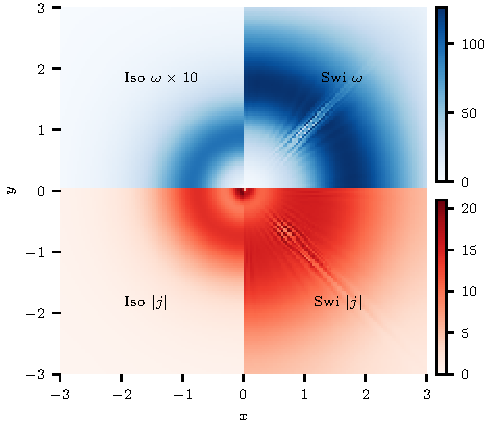
\includegraphics[width=0.48\linewidth]{v-4r-4_vorticity_current_ring_t_9}
  \caption{Note we have multiplied the isotropic vorticity (upper left) by ten to allow comparison.}%
  \label{fig:v-4r-4_vorticity_current_ring_t_9}
\end{figure}

\begin{figure}[t]
  \centering
  \includegraphics[width=0.9\linewidth]{v-4r-4_reconn_rate_swi_t_10.pdf}
  \caption{}%
  \label{fig:v-4r-4_reconn_rate_swi_t_10}
\end{figure}

TODO Include analysis of null collapse triggered by probable fluting instability

%At $t=11$ the KHI is fully developed. Throughout the preceding times, an inner ring of current density forms and grows in magnitude, seen in both the isotropic and switching cases.

%\begin{figure}[H]
  %\centering
  %\includegraphics[width=0.48\linewidth]{./images/null_point_khi/slices/v-4r-4-switching_Velocity_Vz_z_0.0_0011.pdf}
%\end{figure}

%\begin{figure}[H]
  %\centering
  %\includegraphics[width=0.48\linewidth]{./images/null_point_khi/slices/v-4r-4-isotropic_magnitude_current_density_z_0.0_0011.pdf}
  %\includegraphics[width=0.48\linewidth]{./images/null_point_khi/slices/v-4r-4-switching_magnitude_current_density_z_0.0_0011.pdf}
%\end{figure}

%At $t=13$ the null shows some indication of beginning to reconnect and collapse, shown by the presence of velocity structures around the spine, mainly in the isotropic case. The inner ring of current density has shrunk and is now extremely strong, stronger in the isotropic case than the switching case, although we note the current structure located along the spine is around twice as strong as that around the null.

%\begin{figure}[H]
  %\centering
  %\includegraphics[width=0.48\linewidth]{./images/null_point_khi/slices/v-4r-4-isotropic_Velocity_Vx_x_0.0_0013.pdf}
  %\includegraphics[width=0.48\linewidth]{./images/null_point_khi/slices/v-4r-4-switching_Velocity_Vx_x_0.0_0013.pdf}
%\end{figure}

%\begin{figure}[H]
  %\centering
  %\includegraphics[width=0.48\linewidth]{./images/null_point_khi/slices/v-4r-4-isotropic_magnitude_current_density_z_0.0_0013.pdf}
  %\includegraphics[width=0.48\linewidth]{./images/null_point_khi/slices/v-4r-4-switching_magnitude_current_density_z_0.0_0013.pdf}
%\end{figure}

%At $t=14$ in only the isotropic case the ring of density has shrunk entirely to the null.

%\begin{figure}[H]
  %\centering
  %\includegraphics[width=0.48\linewidth]{./images/null_point_khi/slices/v-4r-4-isotropic_magnitude_current_density_z_0.0_0014.pdf}
  %\includegraphics[width=0.48\linewidth]{./images/null_point_khi/slices/v-4r-4-switching_magnitude_current_density_z_0.0_0014.pdf}
%\end{figure}

%At this time, the reconnection rate becomes highly negative at the centre of the plot, in both cases:

%\begin{figure}[H]
  %\centering
  %\includegraphics[width=0.48\linewidth]{./images/null_point_khi/field_line_integrator/v-4r-4-isotropic_integrated_pef_0014.pdf}
  %\includegraphics[width=0.48\linewidth]{./images/null_point_khi/field_line_integrator/v-4r-4-switching_integrated_pef_0014.pdf}
%\end{figure}

%Indeed, by $t=15$, the null is showing signs of collapse in the vorticity, the velocity and in a sudden decrease in current density at the null in the isotropic case.  Note the KHI is still present and the sheer size of the vorticity in the switching case (probably due to a numerical issues, we don't have much stabalising viscous damping in this simulation). It appears as though the presence of the KHI slows the shrinking of the inner current density ring, slowing the eventual collapse of the null.

%\begin{figure}[H]
  %\centering
  %\includegraphics[width=0.48\linewidth]{./images/null_point_khi/slices/v-4r-4-isotropic_vorticity_density_z_0.0_0015.pdf}
  %\includegraphics[width=0.48\linewidth]{./images/null_point_khi/slices/v-4r-4-switching_vorticity_density_z_0.0_0015.pdf}
%\end{figure}

%\begin{figure}[H]
  %\centering
  %\includegraphics[width=0.48\linewidth]{./images/null_point_khi/slices/v-4r-4-isotropic_Velocity_Vz_z_0.0_0015.pdf}
  %\includegraphics[width=0.48\linewidth]{./images/null_point_khi/slices/v-4r-4-switching_Velocity_Vz_z_0.0_0015.pdf}
%\end{figure}

%\begin{figure}[H]
  %\centering
  %\includegraphics[width=0.48\linewidth]{./images/null_point_khi/slices/v-4r-4-isotropic_magnitude_current_density_z_0.0_0015.pdf}
  %\includegraphics[width=0.48\linewidth]{./images/null_point_khi/slices/v-4r-4-switching_magnitude_current_density_z_0.0_0015.pdf}
%\end{figure}

%\subsection{Qualitative analysis of parameter study}

%The results of the single case shown in section TODO vary strongly with $\eta$. Increasing $\eta$ to $10^{-3}$ produces a null that shows no sign of collapse, in that the Poynting flux appears to be balanced by Ohmic losses [TODO, calculate inputs and outputs]. This remains true even if the KHI is present. The effect of the KHI is to increase Ohmic heating through increased reconnection in the fan plane [TODO show this]. In contrast, decreasing $\eta$ to $10^{-5}$ causes the null to collapse much sooner than in the single case above. Again, this is true regardless of the presence of the KHI.

%In all v-3 isotropic simulations there's an odd spike in every variable. This was also seen in the kink simulations. I assume this is due to small fast waves created during the initial ramp up interacting within the isotropic viscous stress tensor to produce odd effects. It appears to only affect the first time step and slightly increases the viscous heating. Since it doesn't happen in the v-4 simulations, and the results are fairly similar, I trust the behaviour of the v-3 simulations after the spike has passed.

%\begin{figure}[H]
  %\centering
  %\includegraphics[width=0.48\linewidth]{./images/null_point_khi/slices/v-3r-3-isotropic_Velocity_Vz_z_0.0_0001.pdf}
  %\includegraphics[width=0.48\linewidth]{./images/null_point_khi/slices/v-3r-3-switching_Velocity_Vz_z_0.0_0001.pdf}
%\end{figure}

%One major result to note is that decreasing $\eta$ disrupts the KHI. Although the initial instability can be see in the v-3r-5-switching case (below, left), it does not grow and, at any rate, is disrupted by the null collapse which happens much earlier in the low $\eta$ cases, starting between $t=8$ and $9$. Increasing $\eta$ appears to reduce the effect of the boundary, producing a much more radially symmetric KHI (below, right).

%\begin{figure}[H]
  %\centering
  %\includegraphics[width=0.48\linewidth]{./images/null_point_khi/slices/v-3r-3-switching_Velocity_Vz_z_0.0_0009.pdf}
  %\includegraphics[width=0.48\linewidth]{./images/null_point_khi/slices/v-3r-5-switching_Velocity_Vz_z_0.0_0006.pdf}
%\end{figure}

%Throughout many of the simulations $\nu$ does not strongly affect the behaviour in the switching case. The is due to the anisotropic part of the tensor being reasonably weak where it is switched on (i.e. away from the null) and the isotropic part only being switched on only at the null where there isn't appreciable velocity shears.

%At $t=1$ the only difference between each of the parameter runs is the thickness of the Alfv\'en wave at $x=0.85$. This increases with both $\eta$ and $\nu$, appearing at its thinnest in the switching sims at $\eta=10^{-5}$.

%\begin{figure}[H]
  %\centering
  %\includegraphics[width=0.48\linewidth]{./images/null_point_khi/slices/v-3r-5-isotropic_Velocity_Vy_x_0.85_0001.pdf}
  %\includegraphics[width=0.48\linewidth]{./images/null_point_khi/slices/v-3r-5-switching_Velocity_Vy_x_0.85_0001.pdf}
%\end{figure}

%For the isotropic simulations, this correlates with the properties of the vorticity ring which increases in radius with decreasing $\nu$ and slightly with decreasing $\eta$. Decreasing $\eta$ makes the ring appear more diffuse (although this could be a difference in scales TODO check this). The peak vorticity within the ring increases with decreasing $\nu$ and increasing $\eta$.

%\begin{figure}[H]
  %\centering
  %\includegraphics[width=0.3\linewidth]{./images/null_point_khi/slices/v-3r-4-isotropic_vorticity_density_x_0.0_0002.pdf}
  %\includegraphics[width=0.3\linewidth]{./images/null_point_khi/slices/v-4r-4-isotropic_vorticity_density_x_0.0_0002.pdf}
  %\includegraphics[width=0.3\linewidth]{./images/null_point_khi/slices/v-5r-4-isotropic_vorticity_density_x_0.0_0002.pdf}
%\end{figure}

%This correlation remains true until the null collapse begins aroung $t=9$ when large vorticities are generated and a clear trend is no longer present.

%Although the ring of current density that appears alongside the vorticity ring shows a similar increase in radius with decreasing $\nu$ and $\eta$, the strength increases with decreasing $\eta$ and with decreasing $\nu$.

%I.e. $\eta$ goes up, peak vorticity goes up, peak current density goes down. Why? Current density down makes sense, resistivity acts to smooth out currents, but how does it affect the vorticity?

%In the switching case, we find the difference in $\nu$ to be negligible until the KHI starts to appear strongly (i.e. $t=9$). Before this point we see extremely high peaks in vorticity, consistent with the increase in vorticity with $\nu$ seen in the isotropic cases. We also see the same decrease in strength with $\eta$. After the KHI occurs, $\nu$ strongly affects the strength of the vorticity and the current density, with the maximum vorticity generally decreasing with decreasing $\nu$ and similarly for the current density. For large values of $\eta$ (i.e.$10^{-3}$) we find evidence (localised regions of very high vorticity and current density) of the KHI promoting reconnection within the fan plane at $t=10$. This occurs sooner for larger values of $\nu$.

%\begin{figure}[H]
  %\centering
  %\includegraphics[width=0.3\linewidth]{./images/null_point_khi/slices/v-3r-3-switching_vorticity_density_z_0.0_0010.pdf}
  %\includegraphics[width=0.3\linewidth]{./images/null_point_khi/slices/v-4r-3-switching_vorticity_density_z_0.0_0010.pdf}
  %\includegraphics[width=0.3\linewidth]{./images/null_point_khi/slices/v-5r-3-switching_vorticity_density_z_0.0_0010.pdf}
%\end{figure}

%\begin{figure}[H]
  %\centering
  %\includegraphics[width=0.3\linewidth]{./images/null_point_khi/slices/v-3r-3-switching_magnitude_current_density_z_0.0_0010.pdf}
  %\includegraphics[width=0.3\linewidth]{./images/null_point_khi/slices/v-4r-3-switching_magnitude_current_density_z_0.0_0010.pdf}
  %\includegraphics[width=0.3\linewidth]{./images/null_point_khi/slices/v-5r-3-switching_magnitude_current_density_z_0.0_0010.pdf}
%\end{figure}

%By $t=11$ this fan-plane reconnection has also occurred in the $\eta=10^{-4}$ cases. We find it does not occur in the $\eta=10^{-5}$ cases where reconnection at the null occurs sooner than in the other cases, disrupting the fan-plane reconnection.

%We also find this for the one KHI-unstable isotropic case, v-5r-3, where the fan-plane reconnection occurs around $t=14$.

%Generally, for $\eta=10^{-3}$, the reconnection rate varies very little with $\nu$ in all cases, however the presence of the KHI (in either the switching or isotropic cases) enhances reconnection.

%For $\eta=10^{-4}$, increasing $\nu$ decreases the reconnection rate however the overall behaviour of reconnection remains the same as the single case.

%For $\eta=10^{-5}$, the reconnection rate is generally higher than the $10^{-4}$ simulations, particularly along the field lines that intersect the vorticity-current density ring, and along the spine until a reconnection event occurs around $t=10$ in the isotropic cases. The strength of the resultant outflows depend strongly on $\nu$, as does the proceeding reconnection within the rest of the structure, the rate of which is generally higher for weaker viscosity. In the switching case, the initial reconnection event appears sooner and, while the reconnection rate remains relatively constant across the range of $\nu$, lower viscosity does lead to a more violent resultant behaviour.

%Wyper conjectured that with decreased $\eta$ and enough time, the highly twisted field around the spine would be unstable to the kink instability. What we find here is that this part of the field, the most twisted point at around $z=\pm 0.08$ is simply the initial point at which reconnection occurs, causing a cascade of violent reconnection into the rest of the null. It's the increased twist in the spine, caused by a lack of magnetic diffusion, that causes the null to collapse sooner. At this stage in the analysis I can find no evidence of the kink instability in the spine, but the temporal resolution is not so great. I'll run further simulations with more data dumps.

%\subsection{Quantitative Analysis of Parameter Study}

%Plotting the kinetic energies of each of the simulations presents a clear indication of how the parameter choice affects the onset of the KHI in the fan-plane (Figure~\ref{fig:kinetic_energy_over_time_parameter}). As a reminder, the simulations using switching viscosity were unstable to the KHI in all cases, however when $\eta = 10^{-5}$, the instability grows more slowly and appears to be interrupted by the collapse of the null. For the isotropic cases, there was only one parameter choice that resulted in instability; $\eta=10^{-3}, \nu=10^{-5}$. This is summarised in table~\ref{tab:stability}. The stability is reflected in the kinetic energies. For resistivities of $10^{-4}$ and $10^{-3}$ using the switching model, there appears a signature shape indicative of the KHI. This is also seen in the unstable isotropic case, $(10^{-3}, 10^{-5})$. Isotropic cases $(10^{-3}, 10^{-4})$ and $(10^{-4}, 10^{-3})$ show a similar initial increase in kinetic energy, however this does not appear to culminate in instability and we do not notice the small amplitude KHI seen in the low-resistivity switching cases where $\eta=10^{-5}$. Prior to $t\approx 8$) the kinetic energy in these cases appears similar to the fully unstable cases, but with a more shallow gradient. This is due to the lower resistivity allowing the Alfv\'en waves to propagate further away from the spine before interacting in the fan-plane, as can be seen by the location of the vorticity sheets compared in Figure~\ref{fig:low_resistivity_voriticy_ring}.

%\begin{figure}[h]
  %\centering
  %\includegraphics[width=0.48\linewidth]{./images/null_point_khi/slices/v-3r-4-switching_vorticity_density_z_0.0_0006.pdf}
  %\includegraphics[width=0.48\linewidth]{./images/null_point_khi/slices/v-3r-5-switching_vorticity_density_z_0.0_0006.pdf}
  %\caption{Comparison of vorticity ring sizes for $\eta = 10^{-4}$ (left) and $\eta = 10^{-5}$ (right)}
  %\label{fig:low_resistivity_voriticy_ring}
%\end{figure}

%\begin{figure}[h]
  %\centering
  %\includegraphics[width=0.8\linewidth]{./images/null_point_khi/energy_plots/parameter_study/kinetic_energy_over_time.png}
  %\caption{Kinetic energy over time}%
  %\label{fig:kinetic_energy_over_time_parameter}
%\end{figure}

%\begin{table}[]
%\centering
%\begin{tabular}{lllll}
%$\eta$    & $\nu$     & Isotropic Stable? & Switching Stable? &  \\
%\midrule
%$10^{-5}$ & $10^{-5}$ & Y                 & Linear N          &  \\
%$10^{-5}$ & $10^{-4}$ & Y                 & Linear N          &  \\
%$10^{-5}$ & $10^{-3}$ & Y                 & Linear N          &  \\
%$10^{-4}$ & $10^{-5}$ & Y                 & N                 &  \\
%$10^{-4}$ & $10^{-4}$ & Y                 & N                 &  \\
%$10^{-4}$ & $10^{-3}$ & Y                 & N                 &  \\
%$10^{-3}$ & $10^{-5}$ & N                 & N                 &  \\
%$10^{-3}$ & $10^{-4}$ & Y                 & N                 &  \\
%$10^{-3}$ & $10^{-3}$ & Y                 & N                 & 
%\end{tabular}
%\caption{Stability in the isotopic and switching cases across varying $\eta$ and $\nu$. The only unstable isotropic simulation is the one corresponding to $\eta = 10^{-3}, \nu = 10^{-5}$.}
%\label{tab:stability}
%\end{table}

%\subsubsection{Why does the KHI not occur at low resistivity}

%\begin{figure}[h]
  %\centering
  %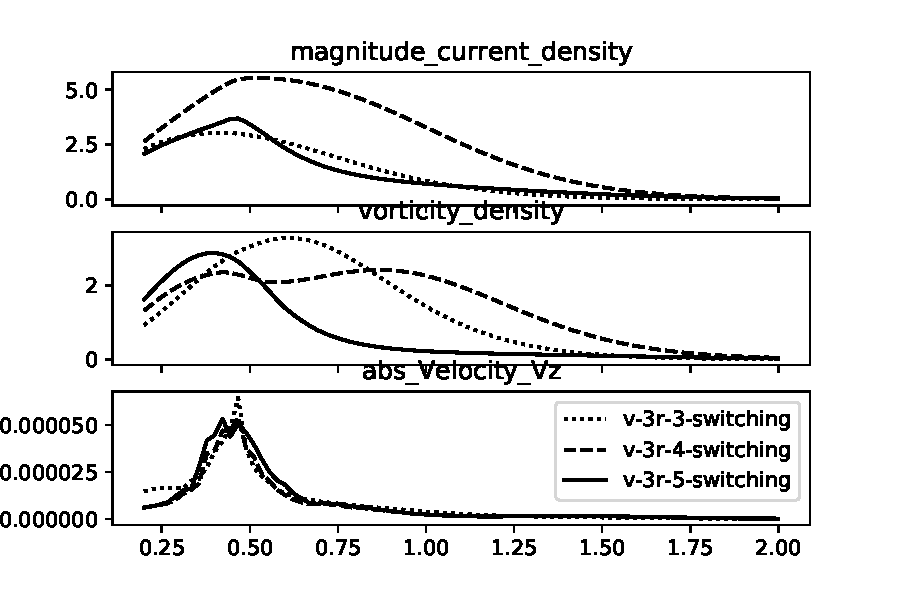
\includegraphics[width=0.8\linewidth]{./images/null_point_khi/azimuthal_averages_v-3_2.pdf}
  %\caption{$t=2$}%
  %\label{fig:azimuthal_averages_v-3_2}
%\end{figure}

%\begin{figure}[H]
  %\centering
  %\includegraphics[width=0.8\linewidth]{./images/null_point_khi/slices/v-3r-5-switching_Velocity_Vz_z_0.0_0002.pdf}
  %\caption{$t=2$}%
  %\label{fig:v-3r-5-switching_Velocity_Vz_z_0_0002}
%\end{figure}

%\begin{figure}[h]
  %\centering
  %\includegraphics[width=0.8\linewidth]{./images/null_point_khi/azimuthal_averages_v-3_4.pdf}
  %\caption{$t=4$}%
  %\label{fig:azimuthal_averages_v-3_4}
%\end{figure}

%\begin{figure}[h]
  %\centering
  %\includegraphics[width=0.8\linewidth]{./images/null_point_khi/azimuthal_averages_v-3_5.pdf}
  %\caption{$t=5$}%
  %\label{fig:azimuthal_averages_v-3_5}
%\end{figure}

%\begin{figure}[h]
  %\centering
  %\includegraphics[width=0.8\linewidth]{./images/null_point_khi/azimuthal_averages_v-3_7.pdf}
  %\caption{$t=7$}%
  %\label{fig:azimuthal_averages_v-3_7}
%\end{figure}

%\begin{figure}[h]
  %\centering
  %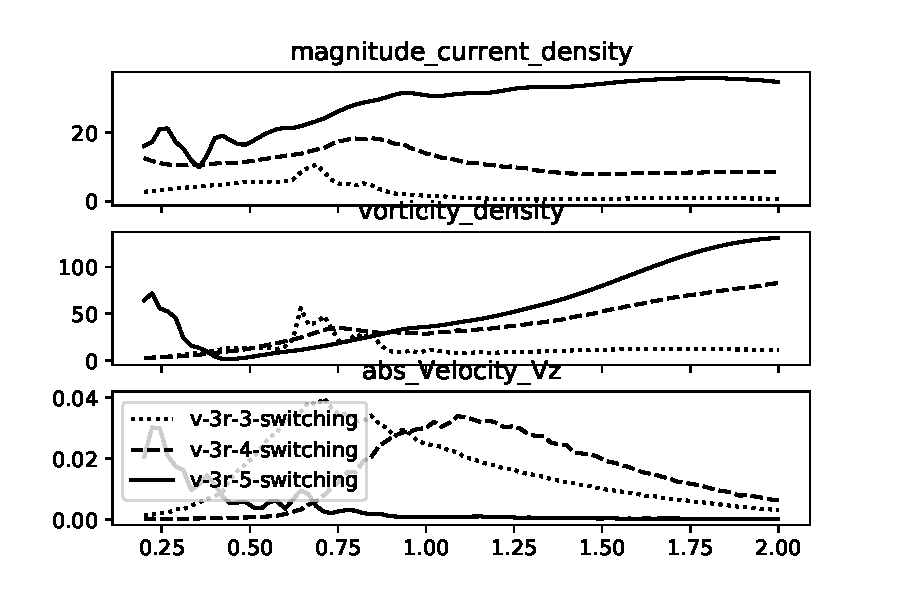
\includegraphics[width=0.8\linewidth]{./images/null_point_khi/azimuthal_averages_v-3_10.pdf}
  %\caption{$t=10$}%
  %\label{fig:azimuthal_averages_v-3_10}
%\end{figure}

%Looking only at the case of $\nu = 10^{-3}$, we can see the KHI appear as early as $t=2$ in the azimuthally averaged velocity in the $z$-direction, for all three values of $\eta$ (Figure~\ref{fig:azimuthal_averages_v-3_2}) and all at approximately the same location, around $r=0.5$. This can also be more clearly seen in the slice through $z$, shown in Figure~\ref{fig:v-3r-5-switching_Velocity_Vz_z_0_0002} for the case $\eta=10^{-5}$, but the pattern is similar for other values of $\eta$. Within only two Alfv\'en times it's clear the KHI is able to grow faster when resistivity is higher, as shown in Figure~\ref{fig:azimuthal_averages_v-3_4} at time $t=4$. After this time the behaviour for each value of $\eta$ diverges. For high and medium values of $\eta$, the initial instability spreads radially, though more slowly in the medium case. The $\eta=10^{-5}$ case shows some evidence of some exchange of energy from the magnetic field to the flow, perhaps caused by a small reconnection event, as can be seen from a small dip in the current density colocating with a sudden and transient increase in velocity (Figure~\ref{fig:azimuthal_averages_v-3_4}). This may also be the point at which the isotropic region switches to the switching region (TODO check). If this is the case, the interpolation between the two regions must be made smoother. At $t=7$ the high resistivity case shows further development of the instability (Figure~\ref{fig:azimuthal_averages_v-3_7}). By $t=10$ (Figure~\ref{fig:azimuthal_averages_v-3_10}) the KHI has grown in both high and medium cases, with the energy of the instability peaking at around $r=0.75$ in the high resistivity case, and $r=1.1$ in the medium case. We also see disruption of the instability before it has properly developed in the low resistivity case.

%\begin{figure}[h]
  %\centering
  %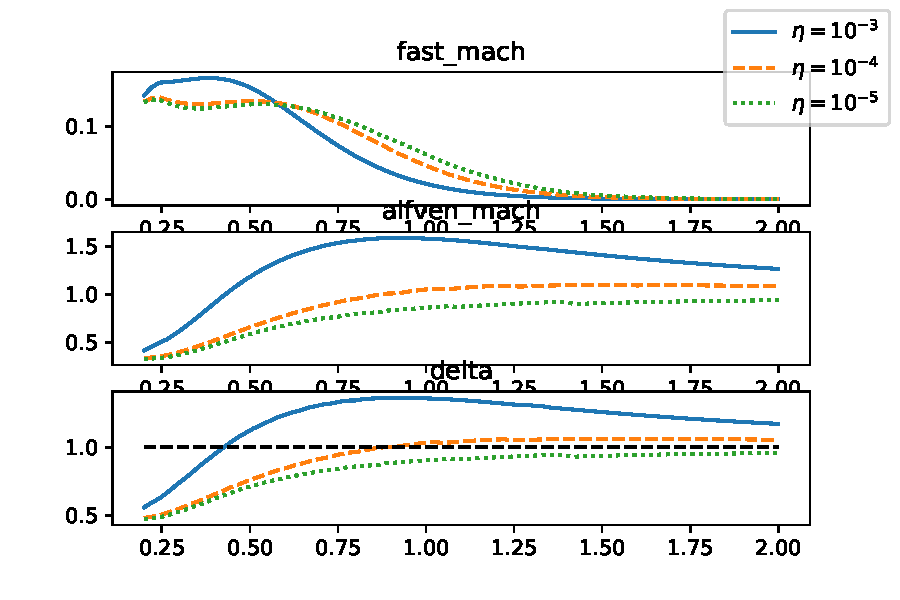
\includegraphics[width=0.8\linewidth]{./images/null_point_khi/mach_numbersv-32.pdf}
  %\caption{Mach numbers at $t=2$}
  %\label{fig:mach_numbersv_32}
%\end{figure}

%\begin{figure}[h]
  %\centering
  %\includegraphics[width=0.8\linewidth]{./images/null_point_khi/mach_numbersv-36.pdf}
  %\caption{Mach numbers at $t=6$}
  %\label{fig:mach_numbersv-36}
%\end{figure}

%It's instructive to study how the relevant Mach numbers and instability parameters vary radially, and link those to the behaviour and stability of the KHI. As an indicator of the stability of the shear layer, we plot the Mach number associated with the fast-mode $M_f = \frac{\Delta v}{\sqrt{c_s^2 + c_A^2}}$, where $\Delta v$ is the difference in velocity over the shear layer, and $c_s$ and $c_A$ are the local sound and Alfv\'en speeds, respectively, as well as the parameter $\Delta = \frac{L_B}{L_v}(M_{A, proj})^{2/3}$, where $L_B$ and $L_v$ are the widths of the respective magnetic and velocity shear layers, and $M_{A, proj}$ is the Alfv\'en velocity of the layer after removing the guide field, i.e. $M_{A, proj} = \frac{\Delta v \sqrt{\rho}}{\Delta B}$ (TODO reword this entire sentence). For the layer to be unstable to the KHI, $M_f < 2$ and $\Delta > 1$. At early times ($t=2$) the initial growth of the instability occurs at $r=0.5$, coinciding with the peak of $M_f$ (Figure~\ref{fig:mach_numbersv_32}). At this time and location, it is only the high resistivity case which shows shear layers with $\Delta > 1$. Both lower resistivity cases are linearly stable to the instability. This changes for the mid resistivity case (TODO decide mid or medium) only around $t=6$ (Figure~\ref{fig:mach_numbersv-36}), where the peak of $M_f$ coincides with the point where $\Delta \approx 1$ and the instability begins to grow.


%\subsection{Parameter study}

%A parameter study was run, varying $\nu$ over three values ($10^{-5}$, $10^{-4}$ and $10^{-3}$), and varying $\eta$ over the same three values, giving nine parameter sets in total. For each of these, two simulations were run, one using the isotropic model and the other using the switching model.

%**General results**

%There are some features common to all simulations: the initial interaction of the twisting motion, resultant counterflows, and the eventual collapse of the null. Initially we observe torsional Alfv\'en waves propagating from the upper and lower footpoints along the field and into the fan plane. The counterflows present in~\cite{wyperKelvinHelmholtzInstabilityCurrentvortex2013} are also seen at $t=3$ TODO PLOT. Much later in the evolution (depending on the value of $\eta$) the null begins to collapse during a period of intense reconnection PLOTS TODO.

%The Kelvin-Helmholtz instability only occurs in those simulations with suitably low viscosity, and a suitable (TODO what is suitable?) early-time counterflow. These conditions are met in all switching cases, except when $\eta=10^{-5}$, and only in the isotropic case of $\nu = 10^{-5}, \eta=10^{-3}$. In all KH unstable cases, the initial instability is seen early, around $t=1$ PLOT TODO, and peaks around $t=10$ TODO CHECK THIS. The evolution takes different forms for different values of $\eta$ and $\nu$.

%- The nature of the reconnection is violent and produces a great deal of Ohmic heating
%- The time at which the reconnection occurs isn't hugely affected by the form and strength of viscosity. The major factor affecting the onset time is the resistivity; the lower the value, the sooner the onset.
%- The resistivity seems to control when reconnection starts; the lower the resistivity the sooner the reconnection begins
%- For low ($\eta=1e-5$) resistivity the KHI in the usually unstable switching case is disrupted. Interestingly, it's not the eventual reconnection that disrupts, but the instability isn't even able to start. It's not clear why.
